%\documentclass[10pt, twocolumn]{article}
\documentclass[twocolumn,showpacs,preprintnumbers,amsmath,amssymb,prd]{revtex4}
%\documentclass[11 pt,preprint,preprintnumbers,amsmath,amssymb, prd]{revtex4}

% Preamble adapted from Surjeet Rajendran

\usepackage{latexsym}
\usepackage{amssymb}
\usepackage{epsfig,amsmath,graphics}
\usepackage{epstopdf}
\usepackage{verbatim}
\usepackage{wasysym}
\usepackage{hyperref}
\usepackage{feynmp-auto} % feynman diagrams
%\usepackage{subfig}
\usepackage[utf8]{inputenc}
\usepackage{xpatch}
\usepackage{xcolor}
\hypersetup{
    colorlinks,
    linkcolor={red!80!black},
    citecolor={green!60!black},
    urlcolor={blue!60!black}
}
\usepackage{appendix}

\newcommand{\Ez}{\mathcal{E}_0}
\newcommand{\Eboom}{\mathcal{E}_\text{boom}}

\newcommand{\OO}{\mathcal{O}}
\newcommand{\LL}{\mathcal{L}}
\newcommand{\HH}{\mathcal{H}}

\newcommand{\TeV}{\text{TeV}}
\newcommand{\GeV}{\text{GeV}}
\newcommand{\MeV}{\text{MeV}}
\newcommand{\keV}{\text{keV}}
\newcommand{\rad}{\text{rad}}
\newcommand{\cm}{\text{cm}}
\newcommand{\angstrom}{\buildrel _{\circ} \over {\mathrm{A}}}
\newcommand{\pslash}{p\hspace{-0.070in}/\,}
\newcommand{\Mpl}{M_{\text{pl}}}
\newcommand{\ket}[1]{\ensuremath{\left|#1\right>}}
\newcommand{\bra}[1]{\ensuremath{\left<#1\right|}}
\newcommand{\braket}[2]{\ensuremath{\left<#1|#2\right>}}
%Large Parentheses
\def\r{\right)}
\def\l{\left(}

\begin{document}

\title{White Dwarfs as Dark Matter Detectors}

\author{Ryan Janish}
\affiliation{Berkeley Center for Theoretical Physics, Department of Physics,
University of California, Berkeley, CA 94720, USA}

\author{Vijay Narayan}
\affiliation{Berkeley Center for Theoretical Physics, Department of Physics,
University of California, Berkeley, CA 94720, USA}

\author{Surjeet Rajendran}
\affiliation{Berkeley Center for Theoretical Physics, Department of Physics,
University of California, Berkeley, CA 94720, USA}

\author{Paul Riggins}
\affiliation{Berkeley Center for Theoretical Physics, Department of Physics,
University of California, Berkeley, CA 94720, USA}

\begin{abstract}

White dwarfs can serve as detectors for ultra-heavy dark matter states which interact to trigger type Ia supernovae.
This was originally proposed in \cite{Graham:2015apa} and used to place bounds on primordial black holes.
In this paper, we extend the reach of white dwarf detectors to dark matter candidates with non-gravitational couplings that release energy in the form of standard model particles.
This is used to constrain dark matter models which can ignite white dwarfs through annihilations, decays, or transits.
As a concrete example, we are able to constrain supersymmetric Q-ball dark matter in a vast region of parameter space fundamentally inaccessible to terrestrial-based experiments.


\end{abstract}
\maketitle
\tableofcontents
\newpage

\section{Introduction}
\label{sec:Introduction}

The detection of ultra-heavy dark matter (DM) is an open problem which will likely require a confluence of astrophysical probes.
For instance, DM masses above $\sim 10^{22} ~\GeV$ will register fewer than a single event per year in a typical terrestrial detector of size $\sim (100 ~\text{m})^2$.
Furthermore, the lack of conclusive signatures on a variety of experimental fronts has led many to consider DM candidates far above the weak scale and their potential signatures \textcolor{blue}{cite}.
One possibility proposed by \cite{Graham:2015apa} is that ultra-heavy DM can trigger supernovae (SN) in sub-Chandrasekhar white dwarf (WD) stars by inducing runaway fusion.
As such, white dwarfs can serve as detectors for ultra-heavy DM states.

White dwarfs are particularly suited to this task as they are more susceptible to runaway fusion than are main-sequence stars.
Runaway fusion requires that two criteria be met: a region within the star must be hot enough to support exothermic fusion reactions, and the rate at which energy is released must dominate any cooling mechanisms that drain energy from the fusing region.
Since the pressure of a WD is set by electron degeneracy and is thus independent of temperature, thermal expansion is suppressed as a potential cooling mechanism.
Therefore WD cooling relies on thermal diffusion, which becomes less important over longer length scales, and can be overcome by sufficiently heating a large enough region of the WD.

The necessary trigger for runaway fusion was initially computed in \cite{Woosley} and recently implemented in \cite{Graham:2015apa} to place bounds on primordial black holes. 
In addition, the authors of \cite{Graham:2015apa} identify several other heating mechanisms involving DM which may be constrained in a similar manner.
In this paper, we extend the reach of WD detectors to DM candidates with non-gravitational couplings which release energy in the form of high-energy standard model (SM) particles.
DM models with interactions of this sort include Q-balls found in supersymmetric extensions of the SM and dark nuclei with higher-dimension couplings to the SM \textcolor{blue}{cite}.
An essential ingredient in this analysis is an understanding of how individual SM particles deposit energy in a WD medium through strong and electromagnetic interactions. 
In this regard, the WD may be thought of as a detector with hadronic and electromagnetic ``calorimeter'' components.
This is used to constrain DM models which can ignite WDs via DM-DM collisions, DM decays, or transits with a DM-SM scattering interaction. 
The resulting constraints will come from either observing specific, long-lived white dwarfs or comparing the measured type Ia SN rate with the expected rate due to DM events.
The former can be viewed as a ``flux is too low" fundamental limit for the WD detector, while the latter can be viewed as a ``detection threshold" for signal over background.  
As a concrete example, we are able to constrain Q-ball DM in regions of parameter space fundamentally inaccessible to terrestrial experiments.
However, it is important to note that any such DM constraints are by nature complimentary to terrestrial ones - it is more massive DM that is likely to trigger SN, and also more massive DM that has sufficiently low flux on Earth.
What allows the WD detector to be effective in this regime is its enhanced surface area $\sim (10^4 ~\text{km})^2$, exceptionally long lifetime $\sim \text{Gyr}$, and astronomical abundance in the galaxy. 

We begin in Section~\ref{sec:Review} by reviewing the mechanism of runaway fusion in a WD. 
The ability for DM to trigger SN through non-gravitational interactions is ultimately based on the heating properties of ordinary SM particles, which is summarized in Section~\ref{sec:SMHeating} for different species and energies.
In Section~\ref{sec:DMexplode} we derive conditions on the properties of DM necessary to ignite white dwarfs, and in Section~\ref{sec:Constraints} we constrain DM models with interactions parameterized by a simple, schematic form.  
We examine the specific case of Q-balls in Section~\ref{sec:QBalls}, and conclude in Section~\ref{sec:Discussion}.

\section{White Dwarf Runaway Fusion}
\label{sec:Review}

Any process which deposits energy in a WD will eventually heat a localized region within the star. 
Since we are interested in nuclear fusion, let $L_0$ be the length scale of the local peak in ion temperature $T_0$ and $\Ez \sim T_0 n_\text{ion} L_0^3$ be the excess thermal energy it contains, where $n_\text{ion}$ is the number density of ions. 
Note that the size and thermal properties of any heated region will evolve in time, so we take $L_0$ and $\Ez$ to characterize this peak as it initially forms, i.e.\ immediately after a temperature profile for ions has been established.
Thus for a given heating event, $L_0$ is a measure of the efficiency with which the energy deposit is transferred to ions in the stellar medium.
This may vary significantly with the form of the energy deposit and with WD density.
For example, suppose that kinetic energy is transferred directly to a single ion through a short-range elastic scatter.
This ion would thermalize with neighboring ions, resulting in a heating length $L_0$ of order the ion mean free path.
In the other extreme, suppose that a process produces electrons in the WD at energies just above the Fermi energy.
These electrons have Pauli-suppressed interactions and will travel a long distance before their energy is scattered and thermalized among ions, resulting in a much larger $L_0$.

The fate of a locally heated region in a WD is either a nonviolent diffusion of the energy deposit across the star, or a runaway fusion chain-reaction that will destroy the star.
The precise outcome is governed by two parameters: the fusion temperature $T_f$ and trigger size $\lambda_T$.
The fusion temperature $T_f$ is the threshold for the onset of fusion and is given by the energy required for ions to overcome their mutual Coulomb barrier.
In carbon-oxygen WDs, this is a constant $T_f \sim \MeV$. \textcolor{blue}{cite}
However, while any region with $T_0 > T_f$ will initially support fusion, this condition is not sufficient for triggering a runaway process.
Sustained heating through nuclear fusion can only be maintained if the timescale for cooling is consistently longer than the timescale for heating. 
Cooling in a WD is dominated by diffusion \textcolor{blue}{cite} and the characteristic diffusion time for a heated region increases with its size while the rate of fusion is independent of size. 
Therefore, there will always be a critical size of a heated region (at fixed temperature) above which fusion is maintained as the dominant thermal process.
For a region at the threshold of nuclear fusion $T_f$, this condition defines the trigger size $\lambda_T$.
The value of $\lambda_T$ is highly dependent on stellar density, and is set by either the thermal diffusivity of photons or degenerate electrons.
It has been calculated numerically in \cite{Woosley} and analytically scaled for varying WD masses in \cite{Graham:2015apa}.
As in \cite{Graham:2015apa}, we restrict our attention to carbon-oxygen WDs in the upper mass range $\sim 0.7 - 1.4 ~M_{\odot}$ which correspond to a central number density of ions $n_\text{ion} \sim 10^{29} - 10^{32} ~\cm^{-3}$.
Over this range, the trigger size is approximately $\lambda_T \sim 10^{-5} - 10^{-2} ~\text{cm}$.

In summary, a local temperature peak $T_f$ in a WD will either always be dominated by diffusive cooling if $L_0 < \lambda_T$ or sustained fusion if $L_0 > \lambda_T$.  
However, there is an additional possibility if $T_0 > T_f$ that the thermal evolution is initially dominated by diffusion but at a later time results in runaway fusion. 
We can assess this outcome by assuming the region with $T_0 > T_f$ begins to diffuse and cool until its temperature reaches $\sim T_f$.
If the size of the region at this point is larger than $\lambda_T$, a runaway will occur.  
For a heated region of initial size $L_0$ and total energy deposit $\Ez$, the condition to trigger a type Ia SN via runaway fusion is
\begin{equation}
\label{eq:boom}
  \Ez \gtrsim n_\text{ion} T_f \text{max}\{L_0, \lambda_T\}^3.
\end{equation}
This implies the explosion condition used in \cite{Graham:2015apa}, but also provides a less stringent criteria applicable to regions of temperature greater than $T_f$ and size less than $\lambda_T$ which was not needed in that work.  
Thus there is an absolute minimum energy required to ignite a WD
\begin{equation}
\label{eq:Eboom}
\mathcal{E}_{\text{boom}} \sim n_\text{ion} T_f \lambda_T^3 \sim 10^{15} - 10^{22} ~\GeV,
\end{equation}
where $\mathcal{E}_{\text{boom}} $ varies with trigger size $\lambda_T$ over the range of WD densities.
This is plotted in Figure \ref{fig:Eboom}.
Note that the threshold \eqref{eq:Eboom} is only sufficient if the deposited energy thermalizes within a region of size $L_0 < \lambda_T$.
The threshold energy for explosion is parametrically larger if energy is deposited on a larger length scale $L_0 > \lambda_T$.
As a result, understanding the heating length $L_0$ of a process is critical to determining whether or not it is capable of destroying a WD. 
\begin{figure}
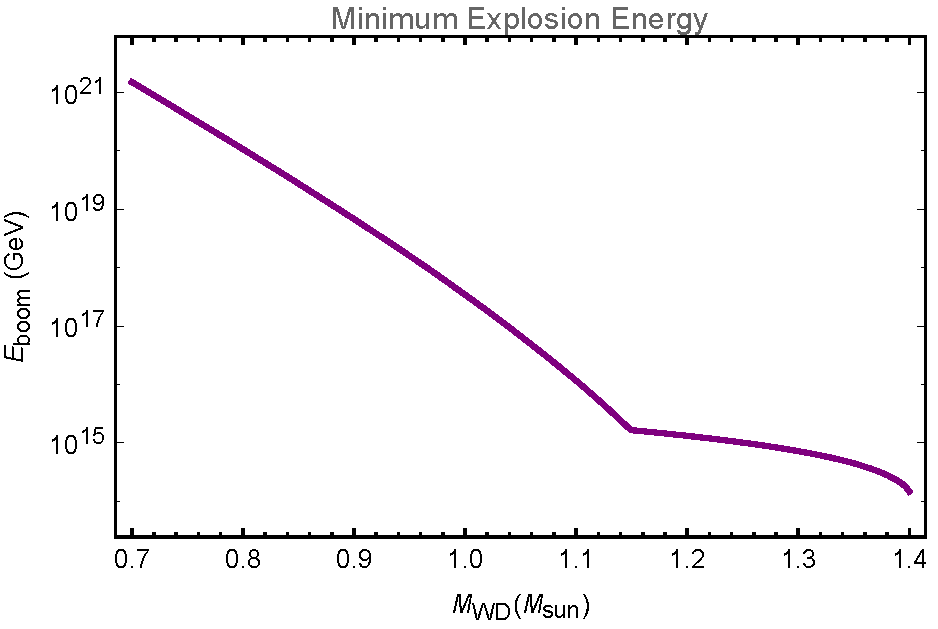
\includegraphics[scale=.45]{Eboom.pdf}
\caption{Minimum energy $\Eboom$ required to trigger SN as a function of WD mass, based on numerical results for $\lambda_T$ \cite{Woosley}.}
\label{fig:Eboom}
\end{figure}

\section{Dark Matter and Non-Gravitational Heating of White Dwarfs}
\label{sec:SMHeating}

Having reviewed the requirements for runaway fusion in a WD, we turn now to the question of triggering these events with a DM encounter. 
This amounts to understanding the heating length $L_0$ and energy deposit $\Ez$ due to a given DM-WD encounter - if these satisfy condition \eqref{eq:boom}, then the encounter is explosive.
Of course, the heating parameters $L_0$ and $\Ez$ necessarily depend on the nature of the DM and must be explicitly calculated for a given DM model. 
This was done in \cite{Graham:2015apa} for primordial black holes, which deposit energy through dynamical friction while transiting the star.
However, non-gravitational interactions also have the potential to trigger SN. 
In particular, any DM candidate which couples to the SM will generically be able to release SM secondaries in the star, which then thermalize with the stellar medium. 
DM encounters that heat the star through this SM-mediated mechanism will be the focus of this work. 
For these processes, the unknown DM physics serves only to determine the initial distribution of the SM particles produced in the star, while the heating proceeds entirely though known SM interactions. 
It is therefore necessary to understand how energy is transferred from SM particles to the stellar medium in order to assess the explosiveness of these encounters, so the remainder of this section is dedicated to computing the heating properties of SM particles.

To focus the calculation, it will be helpful to consider some general properties that the DM-WD encounter must have in order to successfully initiate runway fusion.
We focus on ultra-heavy DM candidates - if the energy of the secondaries is sourced from the DM's kinetic or mas energy, then $m_\text{DM} \gtrsim \Eboom$ for ignition. 
It is possible that this energy is sourced from the stellar medium instead, in which case there is no fundamental limit on $m_\text{DM}$ needed for ignition, but in practice this mass will likely need to be large in order to achieve a DM-SM interaction cross-section sufficient for ignition.
While still distant from the star, the DM will have the galactic viral velocity of $10^{-3}$, but as it passes through the star this will be accelerated to the WD escape speed, $v_\text{esc} \sim 10^{-2}$.
If the DM then interacts to release $N$ particles of typical energy $\epsilon$, we require $\epsilon \gtrsim T_f$ and $N \epsilon \gtrsim \Eboom$.
We are thus sensitive to a GUT-mass or heavier DM particle, likely a complex composite state, which interacts in the WD to produce either have a few GUT-scale SM particles or a very large number of collier-scale particles. 
\textcolor{blue}{We also assume a nominal upper bound $\sim 10^{17} ~\GeV$ so that we may conservatively ignore interactions beyond the SM.} 
The lightest SM states will be most typically produced, so for simplicity we consider only the release of electrons, photons, pions, and nucleons, though the heating due to heavier species is straightforward to determine following the approach used below.
These light secondaries are typically very relativistic, with the exception being the least-energetic hadrons that we consider, with $v \gtrsim 10^{-2}$.
Since this speed is never significantly less the DM velocity, and the ultra-heavy DM carries the bulk of the momentum in the interaction which produces the secondaries, we can to $\OO(1)$ take the momentum of the released SM particles to be isotropic. 

With the above picture in mind, we then consider a primitive process that releases isotropically from a point in the WD interior $N$ particles of SM species $i$, each with energy $\epsilon$, and compute the width $\Delta_i(N, \epsilon)$ of the resulting ion temperature peak. 
If the interaction indeed has this form, then the heating length is given simply by $L_0 \sim \Delta$. 
In a more realistic interaction, however, with the SM secondaries produced according to some distribution in energy and species, one can find $L_0$ either by identifying the strongest-interacting subset of secondaries that carries $\OO(1)$ of the energy, or use an appropriate average of $\Delta$s. 
To compute $\Delta$ for a given $N$, $\epsilon$, we follow the energy transfer from the initial released particle into ions, possibly through several intermediary species, and identify the length scale over which the ions are thermalized.
Note also that any net displacement of the final ion temperature profile from the point of origin of the SM secondaries is irrelevant for determining ignition. 
If $N$ is large this displacement will be vanishing anyway, but for $N \sim \text{few}$ it could be much larger than $\Delta$, so when applicable we will make note of this special case below. 

\subsection{Summary of Stopping Powers}

An essential ingredient in this calculation is the stopping power $dE/dx$ of SM species with various components of the WD medium. 
Perhaps more directly useful is the range $\lambda$, which is the distance a particle travels before losing $\OO(1)$ of its energy, and is given to $\OO(1)$ by $\lambda \sim E \cdot \l dE/dx \r^{-1}$.
A given particle species will off transfer energy to different species, and so before tracing the thermal path of a particular incident species in detail, it is useful to summarize the dominant energy loss mechanisms as a function of special and energy. 
The ranges of each incident species are plotted in Figure \ref{fig:something}, with the dominant energy loss mechanism indicated.
A more detailed analysis of these stopping powers is provided in Appendix \ref{sec:appendix}. 

At high incident energies, $\epsilon \gtrsim 100~\GeV$, the stopping powers of all species are dominated by nonelastic nuclear collisions that produce hadronic showers. 
Effectively, electrons and photons at this energy behave like hadrons with just a slightly longer mean free path for nuclear collisions, and all species at this energy will transfer $\OO(1)$ of their initial energy into hadronic showers.
Hadrons will remain dominated by these showering processes until the very end of our range, $\epsilon \lesssim 10~\MeV$. 
The behavior of these low-energy hadrons is important for either their direct release, or as the end-state of a hadronic shower. 
Neutral low-energy hadrons are dominated by elastic nuclear scatters which directly thermalize ions, however charged hadrons, depending on their mass, may be dominated instead by Coulomb scattering off of WD electrons.
Thus hadronic showers, which produce a variety of hadron species, will terminate by directly thermalizing both electrons and ions with elastic scatters. 

The stopping powers of electrons is more complicated, and is rightly discussed together with the photon stopping power as these two species are highly coupled. 
Electrons will lose energy via bremsstrahlung, though it is import that this process is suppressed in a WD by several mechanisms.
The screening of ion charge by degenerate electrons is very efficient, and above a critical value of ion density $n_\text{EM} \sim 10^{31} ~\text{cm}^{-3}$ effectually shuts off bremsstrahlung radiation for all energies.  
We thus discuss two cases, $n_\text{ion} < n_\text{EM}$ and $n_\text{ion} > n_\text{EM}$

First we consider the low-density, bremsstrahlung-allowed case.  
At low energies, $\epsilon < \GeV$, electrons are predominately stopped by Coulomb collisions with WD electrons 

First, the LPM effect is important at these densities \textcolor{blue}{cite}.
This flattens the slope of the bremsstrahlung stopping power at high energies, which is what allows the electronuclear nonelastic collisions to dominate at sufficiently large energies.
Bremsstrahlung does become the dominant source of electron stopping for $10~\GeV \lesssim \epsilon \lesssim 1~\TeV$, where it eventually gives way at $\epsilon < 1~\GeV$ to elastic electron-electron Coulomb scattering. 
Photons follow a similar story, becoming dominated by LPM-suppressed electron-positron pair production at intermediate energies $1~\GeV \lesssim \epsilon \lesssim 100~\GeV$, and then elastic Compton scattering off of electrons for $\epsilon \lesssim 1~\GeV$. 

Bremsstrahlung is also suppressed due to the efficient charge screening of ions by degenerate electrons - above a critical value of ion density $n_\text{EM} \sim 10^{31} ~\text{cm}^{-3}$, this effectually shuts off bremsstrahlung radiation for all energies.  and pair production from providing significant energy loss. 



\subsection{Heating Properties - Hadrons}

The stopping powers for nucleons and pions in a WD are shown in Figures \ref{fig:SPnuc} and \ref{fig:SPpion}.
For energies greater than the typical nuclear binding energy $E_\text{nuc} \sim 10 ~\text{MeV}$, the energy loss for light hadrons is dominated by nonelastic nuclear collisions. 
In these collisions the incoming hadron interacts with a single nucleon in the target nucleus, which is converted into several outgoing hadrons.
The remaining nucleus is left in an excited state of energy $\sim E_\text{nuc}$ with negligible center-of-mass recoil. 
Thus incident energies $E \gtrsim E_\text{nuc}$ are to leading order transfered entirely to the secondary hadrons, each of which will carry an $\OO(1)$ fraction of the incident energy.
The outgoing hadrons will be pions and nucleons in roughly equal fractions, along with a few heavier states, i.e.\ deuterons, alpha particles, etc.\ \textcolor{blue}{citation}
If these secondaries have energy above $E_\text{nuc}$, they are alo predominantly stopped by nonelastic nuclear collisions and a roughly collinear hadron shower will result. 
The energy loss of shower constituents is described by the radiative stopping power
\begin{equation}
  \l \frac{dE}{dx} \r \sim \frac{E}{l_\text{h,non}},
\end{equation}
where $l_\text{h,non}$ is the mean free path for nonelastic hadron-nuclei collisions, which is roughly constant over hadron species \textcolor{blue}{citation}.
The shower terminates when constituents reach energies of order $E_\text{nuc}$ so that the shower length induced by an initial hadron of energy $\epsilon$ is approximately 
\begin{align}
\label{eq:hadlength}
  X_\text{h} \sim l_\text{h,non} \log\l\frac{\epsilon}{E_\text{nuc}}\r 
  \sim 10 ~l_\text{h,non}. 
\end{align}

The hadronic shower results in a cloud of light hadrons, each with energy $\sim E_\text{nuc}$. 
The energy loss of these particles is now dominated by elastic scatters, but the target species that receives $\OO(1)$ of the energy depends on the charge of the shower products - charged hadrons will cool by Coulomb scattering electrons, while neutral hadrons will cool by elastic nuclear scatters. 
Charged and neutral hadrons will both carry $\OO(1)$ fractions of the shower energy, so we may ignore the energy that passes into electrons via charged hadrons as this will thermalize ions over a much longer distance than will the neutral hadrons which scatter ions directly. 
Similarly, we focus on the final-state neutrons over the neutral pions, as these thermalize on a slightly shorter distance due to their larger mass. 
Thermalization of the neutrons occurs after they have scattered $\OO(1)$ of their energy, which requires $\sim 10$ hard nuclear collisions. 
Thus during this process the neutrons random walk only a few mean free paths before thermalizing, and so the ions are thermalized over a distance
\begin{align}
  X_\text{n,el} \sim l_\text{h,el}  
\end{align}
where $ l_\text{h,el}$ is the mean free path for elastic nuclear scattering. 

The hadronic shower is mostly collinear, so a single high-energy hadron will produce an ion temperature profile of size $X_\text{n,el}$ that is displaced by $X_\text{h}$ from its starting point. 
If many low-energy hadrons are released and thermalize collectively, they will produce an ion profile centered on their origin with size $X_\text{h} + X_\text{n,el}$.
These two scales are
\begin{align}
  X_\text{h} \sim 10 ~l_\text{h,non}
  &\sim 10^{-6} ~\text{cm} \l\frac{10^{32}~\text{cm}^3}{n_\text{ion}}\r \\ 
  X_\text{n,el} \sim l_\text{h,el}  
  &\sim  10^{-8} ~\text{cm} \l\frac{10^{32}~\text{cm}^3}{n_\text{ion}}\r
\end{align}
where we have used empirically measured cross-sections $\sigma_\text{h,el} \approx 10~\sigma_\text{h,non} \approx 1~\text{barn}$ and conservatively taken these cross-sections to be constant with incoming particle energy.
Note that $X_\text{h}$ dominates in the many-particle case and a more compact heating is achieved with a single high-energy hadron. 
However, both of these scales are below the trigger size for the most massive WDs and so either mechanism will result in ignition with the deposit of the minimal energy $\Eboom$. 

\subsection{Heating Properties - Electrons and Photons}

Released electrons and photons will heat the stellar medium through several distinct channels, depending on the energy of the incident particles and the stellar density.  
Roughly, at high energies $\epsilon \gtrsim 100~\GeV$, both electrons and photons will behave qualitatively as hadrons, producing hadronic showers after interacting with a nucleus via virtual quarks. 
There is then a small window of intermediate energy, $10~\GeV \lesssim \epsilon \lesssim 100~\GeV$, in which the dominant interaction produces EM showers that eventually terminate in a cloud of hot electrons and photons. 
These shower products will first rapidly thermalize into a local, hot electron-photon gas, which then on a much slower timescale heats ions either by electron-ion Coulomb scattering or photonuclear hadronic showers, depending on the temperature of the thermalized shower products. 
Low energy particles $\MeV \lesssim \epsilon \lesssim 10~\GeV$ will not have an EM showering phase, but instead directly thermalize an electron-photon gas through elastic scatters, and then proceed to heat ions as in the intermediate-energy case.  

Finally, the small windows for producing EM showers only occurs in low-density stars, since for very large ion densities, above a critical value $n_\text{EM} \sim 10^{31} ~\text{cm}^{-3}$, charge screening prevents bremsstrahlung and pair production from providing significant energy loss. 
For these WDs, EM showers are a negligible and electrons and photons with $\MeV \lesssim \epsilon \lesssim 100~\GeV$ will all thermalize via elastic scatters as in the low-energy case. 


can essentially be ignored.
We begin by considering WD densities $n_e \lesssim 10^{32} ~\text{cm}^{-3}$.
The electron and photon energy loss functions for a density in this range are shown in Figures \ref{fig:SPelectron} and \ref{fig:SPphoton}.
In the case of both species, the dominant stopping mechanism at incident energies $\epsilon \sim 10^{3}-10^{5} ~\text{MeV}$ is due to electromagnetic radiative processes.
For an incident electron or photon of energy $\epsilon$, this will result in a cascade of secondary electrons and photons with typical shower length
\begin{equation}
X_\text{em} \sim X_0 \l \l \frac{\epsilon}{E_\text{LPM}}\r^{1/2} - \l \frac{E_c}{E_\text{LPM}}\r^{1/2} \r,
\end{equation}
where $X_0$ is the radiation length and $E_\text{LPM}$ is the scale of LPM suppression, defined in Appendix \ref{sec:appendix}.
For an electromagnetic shower, $E_c \sim ~\text{TeV}$ is set by the energy at which Compton scattering dominates the stopping power.
At $\epsilon \sim 10^{5} ~\text{MeV}$, bremsstrahlung is suppressed by $\OO(\alpha)$ due to the LPM effect.

Therefore, at sufficiently high energies $\epsilon \gtrsim 10^5 ~\text{MeV}$ electrons and photons in the WD will lose energy primarily through nuclear interactions.
Effectively, electrons and photons at this energy behave like hadrons and will dump $\OO(1)$ of their initial energies into hadronic showers of length \eqref{eq:hadlength}.
However, the initial distance traversed to trigger a hadronic shower will vary between the two species.
For photons, this is roughly the photonuclear mean free path $l_\gamma$ while for electrons, the ``electronuclear radiation length" is found to be of order $\sim 10  ~l_\gamma/\alpha$.
Note that these initial length scales will dominate the overall size of $L_i$ as compared to the hadronic shower length.
In addition, $L_\text{electron}$ and $L_\text{photon}$ in this energy range also scale roughly linearly with WD density.
We now consider $n_e \gtrsim 10^{32} ~\text{cm}^{-3}$, for which radiative processes are negligible.
In this density regime, the stopping of electrons of incident energy $\epsilon \sim 1 - 10^4 ~\text{MeV}$ is primarily due to Coulomb collisions off degenerate electrons in the star.
At energies $\epsilon \gtrsim 10^4 ~\text{MeV}$, electronuclear and photonuclear processes become the dominant source of energy loss.

\subsection{Summary of Standard Model Heating Channels}

Of course, if the energy deposit required to trigger a SN is greater than $\eqref{eq:coldecay}$ but still less than $\sim 10^{17} ~\GeV$, then it is possible that a single particle containing this energy is sufficient.
This is especially intriguing when we consider collisions or decays that release energy predominantly into neutrinos.
Neutrinos interact very weakly, although their nuclear cross section generically rises with energy.
A highly conservative estimate of this cross section in the energy regime of interest $\sigma_{\nu N} \sim 10^{-34} ~\text{cm}^2$ would indicate a mean free path of order $\sim \text{m}$.
Evidently, the neutrino heating length is too large to consider multiple neutrino emissions within a region of size $\lambda_T$.
However, a single neutrino can be thought of as a displaced vertex of size $\sim \text{m}$ which subsequently transfers its energy into high-energy hadrons or charged leptons.
Therefore, any DM model which admits a annihilation or decay into neutrinos of energy greater than $\sim 10^{15} ~\text{GeV}$ can be constrained just as we are able to do for more strongly interacting SM species.

To summarize, $L_i$ has been computed and plotted in Figure \ref{fig:cash} for the maximal WD density $n_e \sim 10^{33} ~\text{cm}^{-3}$ in the case of hadrons, electrons, and photons.

\section{Dark Matter-Induced Ignition: Conditions}
\label{sec:DMexplode}

In this Section, we parameterize aspects of the DM-induced heating of WDs that are purely dependent on the nature of DM. 
In particular, we derive explosion conditions on DM-WD encounters in terms of their heating lengths $L_0$ that determine whether or not they are capable of igniting the star.
This is done for the three illustrative examples depicted in Figure \ref{fig:feynman}: DM-DM collisions, DM decays, and DM transits. 
\begin{figure}
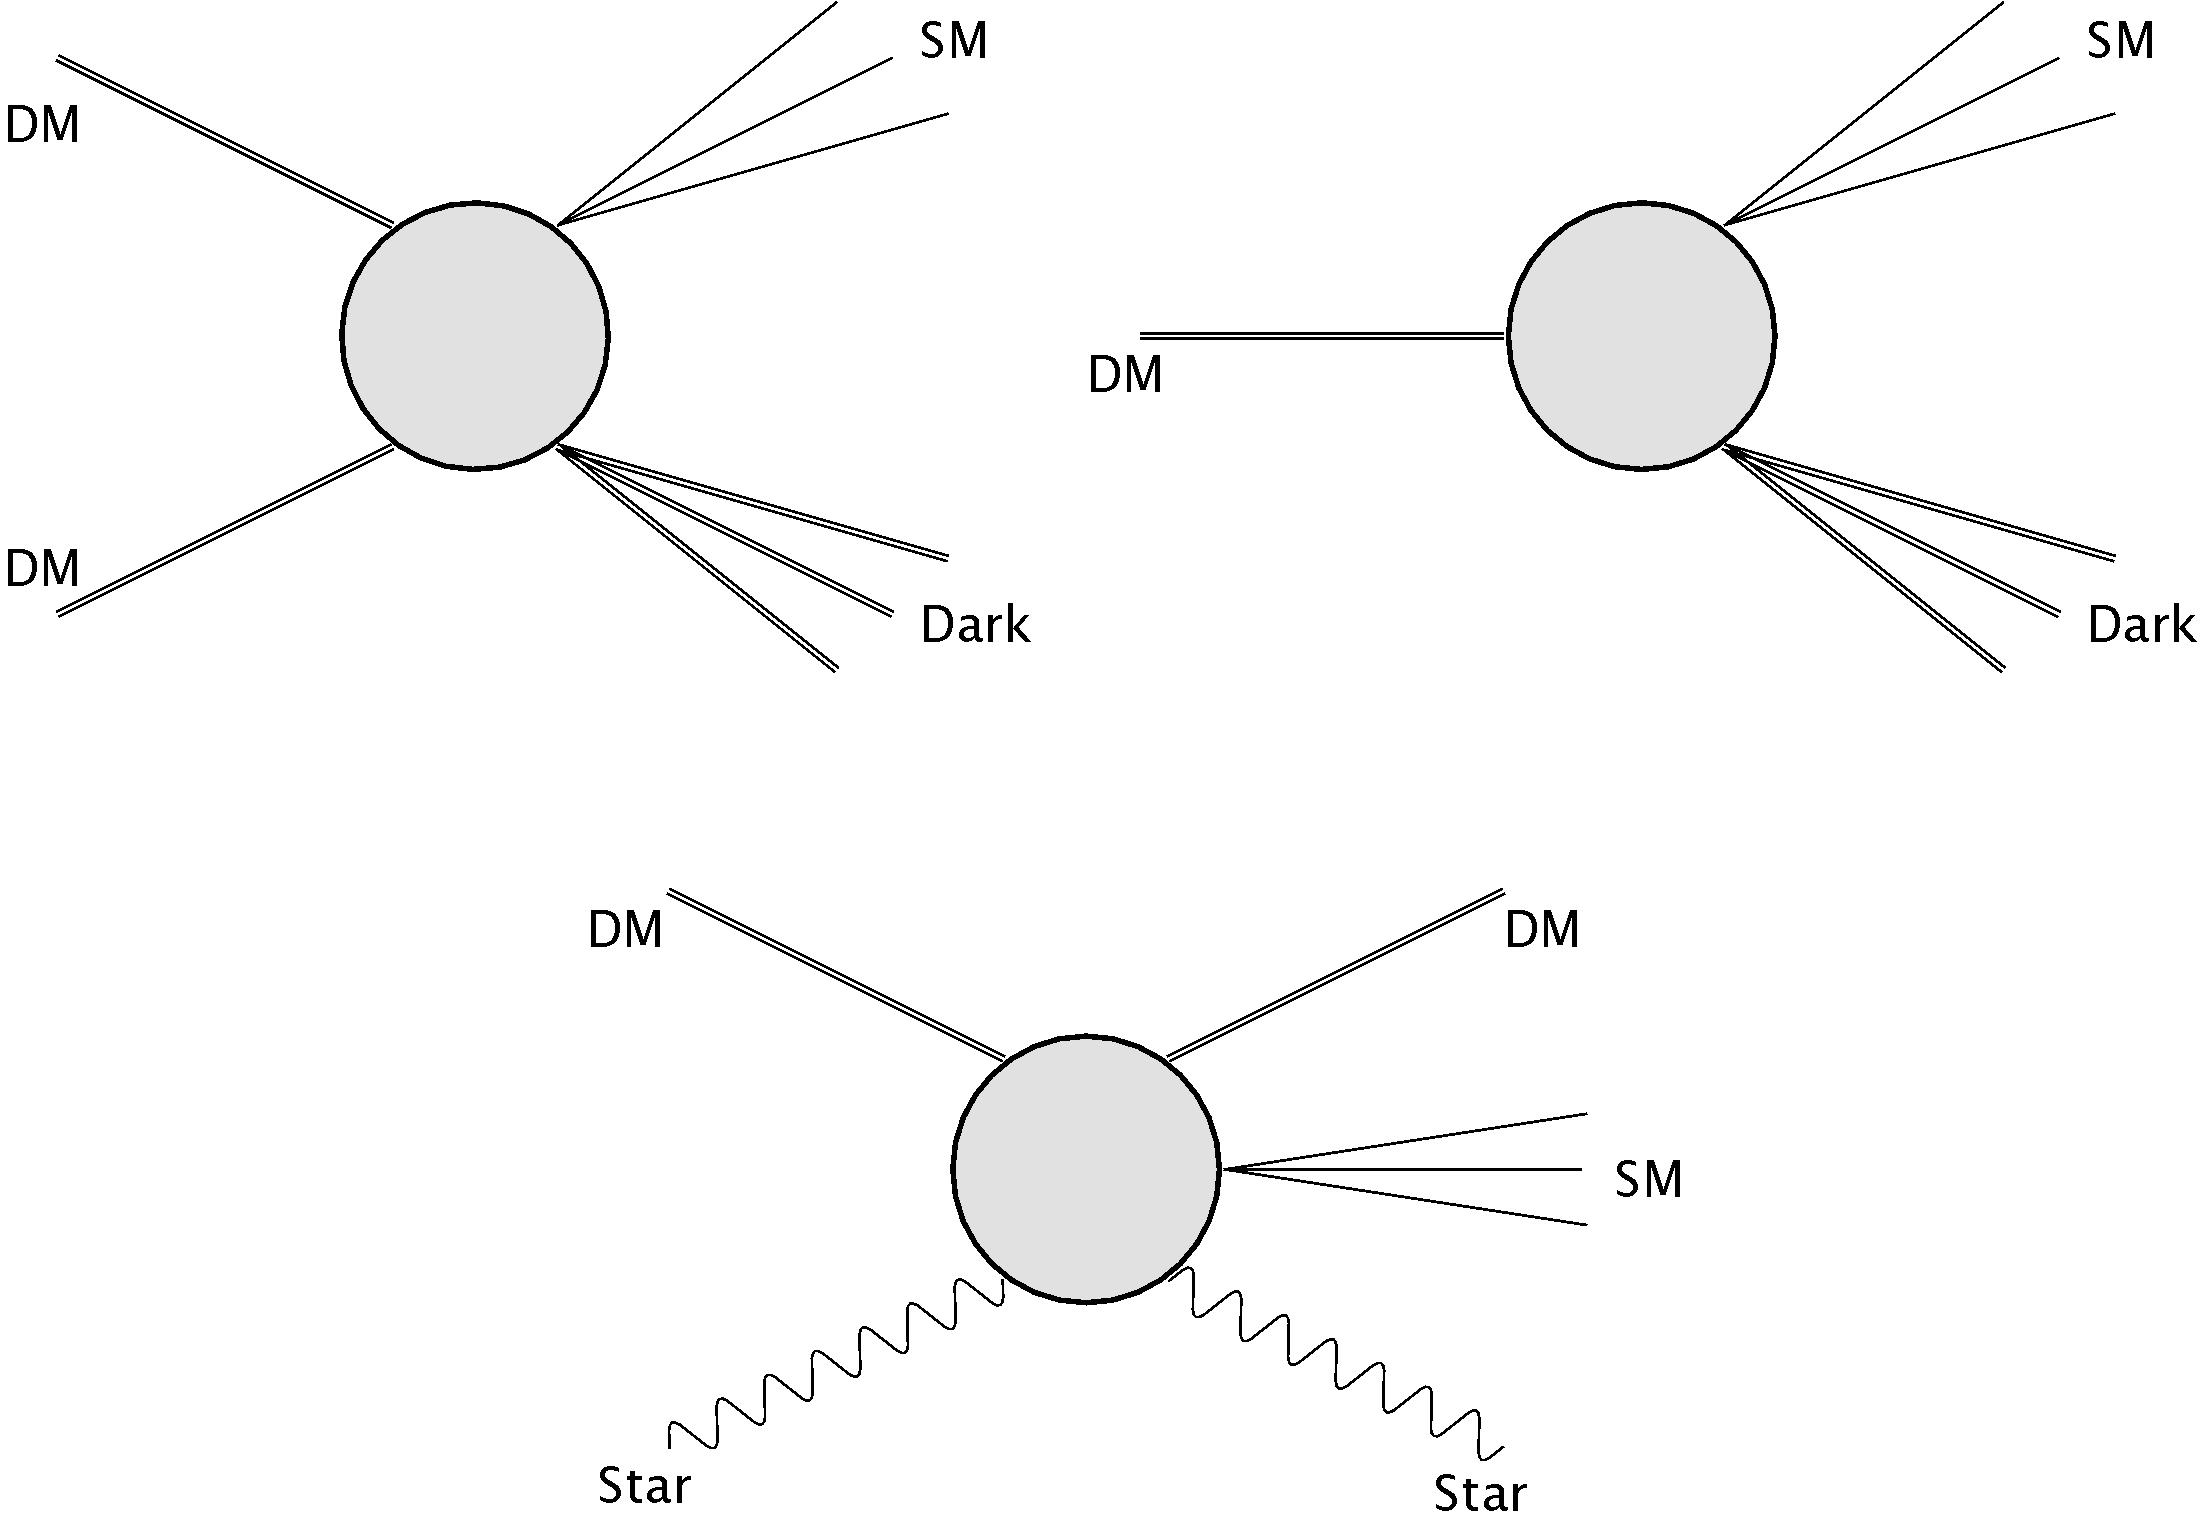
\includegraphics[scale=0.09]{feynmandiag.jpg}
\caption{Schematic of possible non-gravitational DM interactions in a WD. Heating of the WD occurs through SM particle production (also depicted are potential dark sector states involved).}
\label{fig:feynman}
\end{figure}

\subsection{DM-DM Collisions and DM Decays}
\label{sec:DMcoldecay}

The collision of two DM states or the decay of a single DM within the WD is a generic interaction found in many models.
Note that these DM-DM collisions are not necessarily particle-antiparticle annihilations, but can be of a more general, complicated nature such as the collisions of heavy nuclei.
Since any such event will likely result in both SM and dark sector products, we assume the energy released into the SM is a fraction $\eta$ of the DM mass.
%Generically we might expect $\eta \ll 1$, although $\eta$ is at most unity for non-relativistic DM.
For simplicity, we only consider ``point-like" annihilations and decays which release SM particles within a sufficiently localized region. 
This excludes interactions involving the decay of long-lived, meta-stable dark states or other displaced vertices. 
With this parameterization, the explosion condition is approximately the same for both DM-DM collisions and DM decays:
\begin{equation}
\label{eq:coldecay}
    m_\text{DM} \gtrsim \Eboom \cdot \frac{1}{\eta}
      \text{max}\left\{1, \frac{L_0}{\lambda_T}\right\}^3
\end{equation}
Considering the threshold \eqref{eq:Eboom}, such heating events require DM masses larger than $\sim 10^{15} ~\GeV$ in order to release sufficient energy to trigger a SN.

\subsection{DM Transits}
\label{sec:DMdecay}

For DM models with a DM-SM scattering interaction, there may be a continuous release of high-energy SM particles as the DM traverses a WD.
This is parameterized by a linear energy transfer $(dE/dx)_\text{LET}$, which is the energy released into SM products per distance traveled in a WD.
Such a process can be broken up into a series of multiple heating events depositing energy $L_0 (d E/d x)_\text{LET}$ into temperature peaks of size $L_0$, where $L_0$ is the heating length for a single scatter. 
If any individual deposition satisfies \eqref{eq:boom}, then runaway fusion obviously occurs.
If not, a SN may still be triggered due to the combined effect of many deposits.
In such a scenario a large number of nearby temperature peaks will each diffuse outward, eventually merging into an explosive thermal profile satisfying \eqref{eq:boom}.
This is possible if the heating length is smaller than the trigger size $L_0 < \lambda_T$, in which case it is sensible to consider the combined deposit as a single heating event of length $\lambda_T$ and energy $\lambda_T (d E/d x)$.
However, such a coherent addition of individual energy deposits is only possible if the DM transit time is smaller than the relevant thermal evolution timescale.
The latter is dominated by the diffusion time $\tau_d$ across a distance $\lambda_T$ at temperature $T_f$.
Thus we require
\begin{align}
\tau_d \sim \frac{\lambda_T^2}{\alpha(T_f)} \gg \frac{\lambda_T}{v_\text{esc}},
\label{eq:SlowDiffusion}
\end{align}
where $\alpha(T_f)$ is the temperature-dependent diffusivity.
This condition is independent of DM model and has been checked to be satisfied for all WD densities.

In addition, we can parametrize the DM kinetic energy loss per distance travelled in a WD by a DM stopping power $(dE/dx)_\text{SP}$. 
Note that while $(dE/dx)_\text{LET}$ and $(dE/dx)_\text{SP}$ are conceptually related parameters and may be equal in important special cases, they are generically different.
We restrict ourselves to a ``bullet-like" transit in which DM penetrates the non-degenerate crust of a WD with negligible change in kinetic energy
\begin{align}
\label{eq:CrustCondition}
  \left( \frac{d E}{d x} \right)_\text{SP} \ll 
  \frac{m_\text{DM} v^2_\text{esc}}{R_\text{crust}},
\end{align}
where $R_\text{crust} \sim 50 ~\text{km}$ is the width of a WD crust and $v_\text{esc} \sim 10^{-2}$ is the escape velocity of a WD. 
If \eqref{eq:CrustCondition} were not satisfied, then the explosiveness of a transit would be highly dependent on details of the DM stopping power and must be calculated from a specific model.
We avoid this complexity by simply imposing that the DM reaches the degenerate stellar interior, where runaway fusion can be triggered, unimpaired in its initial transit of the star. 
Furthermore, note that $R_\text{crust}$ is many orders of magnitude larger than $\lambda_T$ or any of the heating lengths considered in this work. 
Therefore, the assumption of a DM transit at roughly constant velocity also allows us to ignore DM energy loss within the desired heating region in the WD interior. 
The explosion condition for transits satisfying \eqref{eq:SlowDiffusion} and \eqref{eq:CrustCondition} is given by
\begin{equation}
\label{eq:transitexplosion}
  \left( \frac{d E}{d x} \right)_\text{LET} \gtrsim n_\text{ion} T_f\, \text{max}\left\{\lambda_T, L_0 \right\}^2.
\end{equation}

\section{Dark Matter-Induced Ignition: Constraints}
\label{sec:Constraints}

We now constrain models of DM which will ignite a WD via one of the processes parameterized in Section \ref{sec:DMexplode}.
In order to do so, we additionally assume a simple, schematic form for the DM interactions such that $L_0$ can be calculated exactly using the results of Section \ref{sec:SMHeating}.
However, we first review the different ways in which white dwarfs can constrain DM candidates capable of triggering SN. 

\subsection{Review of WD Constraints}
Following the discussion of \cite{Graham:2015apa}, our constraints come from (1)~the existence of heavy, long-lived white dwarfs, or (2)~the measured type Ia SN rate. 
The typical age of a WD is of order the age of the universe $\sim \text{Gyr}$.
RX~J0648.04418 is a nearby star and one of the heaviest known WDs with a mass $\sim 1.25 ~M_{\odot}$. 
Of course, this is not the only known heavy WD - the Sloan Digital Sky Survey has found $\sim 20$ others. 
The NuStar collaboration has also recently uncovered evidence for the likely existence of $\sim 1.25 ~M_{\odot}$ WDs in the galactic center as well \textcolor{blue}{cite}.
Such candidates are particularly suited for our constraints as the energy deposit needed to trigger supernova is a strong function of WD mass.
However, less dense white dwarfs are significantly more abundant in the galaxy.
Thus, even if a sufficiently massive DM is unable to trigger a violent heating event within the lifetime of a WD, it could still ignite enough lighter WDs to affect the measured SN rate of $\sim $ 0.3 per century.
The DM-induced SN rate is estimated using the expected number of white dwarfs per galaxy $\sim 10^{10}$ and their mass distribution \textcolor{blue}{cite}.
Simulations indicate that only WD masses heavier than $\sim 0.85 ~M_{\odot}$ will result in optically visible SN.
Therefore, most of the stars exploded in this manner will be in the mass range $\sim 0.85 - 1 ~M_{\odot}$, resulting in weaker SN than expected of typical Chandrasekhar mass WDs.

In summary, a bound on DM parameters can be placed if either a single explosive event occurs during the lifetime of an observed star such as RX~J0648.04418 or a possible heavy WD in the galactic center, or the SN rate due to such DM events throughout the galaxy exceeds the measured value.
Note that the energy deposit necessary to trigger SN \eqref{eq:boom} is, in the low-density regime, a strong function of WD density. In \cite{Graham:2015apa} the WD central density was consistently used to describe primordial black hole transits. However, it is found that the WD density changes an $\OO(1)$ fraction from the central value out at a distance $\sim R_\text{WD}/2$ \textcolor{blue}{cite}. Therefore using the central density is a decent approximation as long as we consider heating events within this ``modified" WD volume. For simplicity, we employ this approach.  


\subsection{Collision and Decay Constraints}
\label{sec:CollisionConstraints}

The number of DM particles contained in a WD volume is approximately $\sim n_\text{DM} R_\text{WD}^3 (v_\text{esc}/v)$, taking into account the gravitationally enhanced DM number density within the star.
$v \sim 10^{-3}$ is the virial velocity of DM.
\textcolor{red}{of same order in galactic center?} Therefore, the expected DM-DM collision rate parameterized by cross section $\sigma_\text{DM-DM}$ is 
\begin{equation}
\Gamma_\text{collision} \sim \l \frac{\rho_{\text{DM}}}{m_\text{DM}} \r^2 \sigma_\text{DM-DM} \l \frac{v_\text{esc}}{v}\r^3 v R_\text{WD}^3,
\label{eq:collisiongamma}
\end{equation}
where $\rho_{\text{DM}}$ is the energy density of DM in the region of interest.
For a nearby star we take $\rho_\text{DM} \sim 0.4 ~\GeV/\text{cm}^3$, while for the white dwarfs observed in the galactic center we assume $\rho_\text{DM} \sim 10^3 ~\text{GeV}/\text{cm}^3$.
Likewise, the rate at which a single DM decay event occurs in the WD is
\begin{equation}
\Gamma_\text{decay} \sim  \frac{1}{\tau_\text{DM}} \frac{\rho_{\text{DM}}}{m_\text{DM}} \l \frac{v_\text{esc}}{v} \r R_\text{WD}^3,
\label{eq:taugamma}
\end{equation}
where $\tau_\text{DM}$ is the mean lifetime of DM.

We are able to constrain DM parameters whenever such processes satisfy the explosion condition $\eqref{eq:coldecay}$. 
Consider a schematic interaction where an annihilation or decay releases a number of SM particles $N_i$ of single species $i$ and individual energy $\epsilon$. 
These released particles will deposit their energy and thermalize ions within a heating length explicitly calculated in Section \ref{sec:SMHeating} for hadrons, electrons, and photons.
If we assume a fractional parameter $\eta=1$, this corresponds to the entire mass of DM being converted into SM particles $i$, each with energy $m_\text{DM}/N_i$.
At sufficiently large $\epsilon \gtrsim \text{TeV}$, it has been shown that the heating properties of individual SM particles only varies logarithmically in energy, independent of the species $i$.
Therefore, we treat $\epsilon$ as a free parameter whose precise value above $\sim \text{TeV}$ does not qualitatively modify the limits imposed.
In this case, $N_i$ and $\epsilon$ can both be fixed to the value at which $N_i \epsilon$ is of order $m_\text{DM}$ without affecting the nature of the constraints.
%The only caveat in this scenario is that the value of $L_i (\epsilon)$ extrapolated to energies beyond $\sim 10^{17} ~\GeV$ must be done with caution.
%As a result, for $m_\text{DM}$ greater than this scale, one can simply impose $\epsilon \lesssim 10^{17} ~\GeV$ with the number of released particles necessarily $N_i > 1$.
With the above schematic for DM-DM collisions, we constrain the cross section $\sigma_\text{DM-DM}$ as a function of $m_\text{DM}$ using the different classes of observation available and for representative choices of $\eta$ and SM species $i$ released.
This is done in Figures \ref{fig:collisionclasses}, \ref{fig:collisioneta}, and \ref{fig:collisionspecies}. 
In a similar manner, we constrain the lifetime $\tau_\text{DM}$ as a function of $m_\text{DM}$ in Figures \ref{fig:decayclasses}, \ref{fig:decayepsilon}, and \ref{fig:decayspecies}.

\begin{figure}
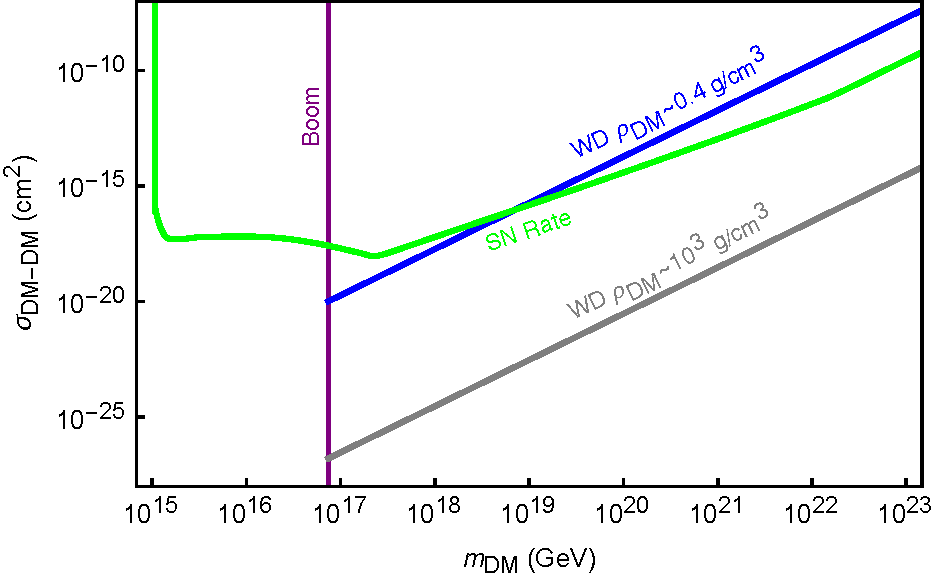
\includegraphics[scale=.45]{collisionobservation.pdf}
\caption{Constraints on DM-DM collision cross section into photons with $\eta =1$. Bounds come from observations of a single WD (local and galactic center) and measured SN rate}
\label{fig:collisionclasses}
\end{figure}

\begin{figure}
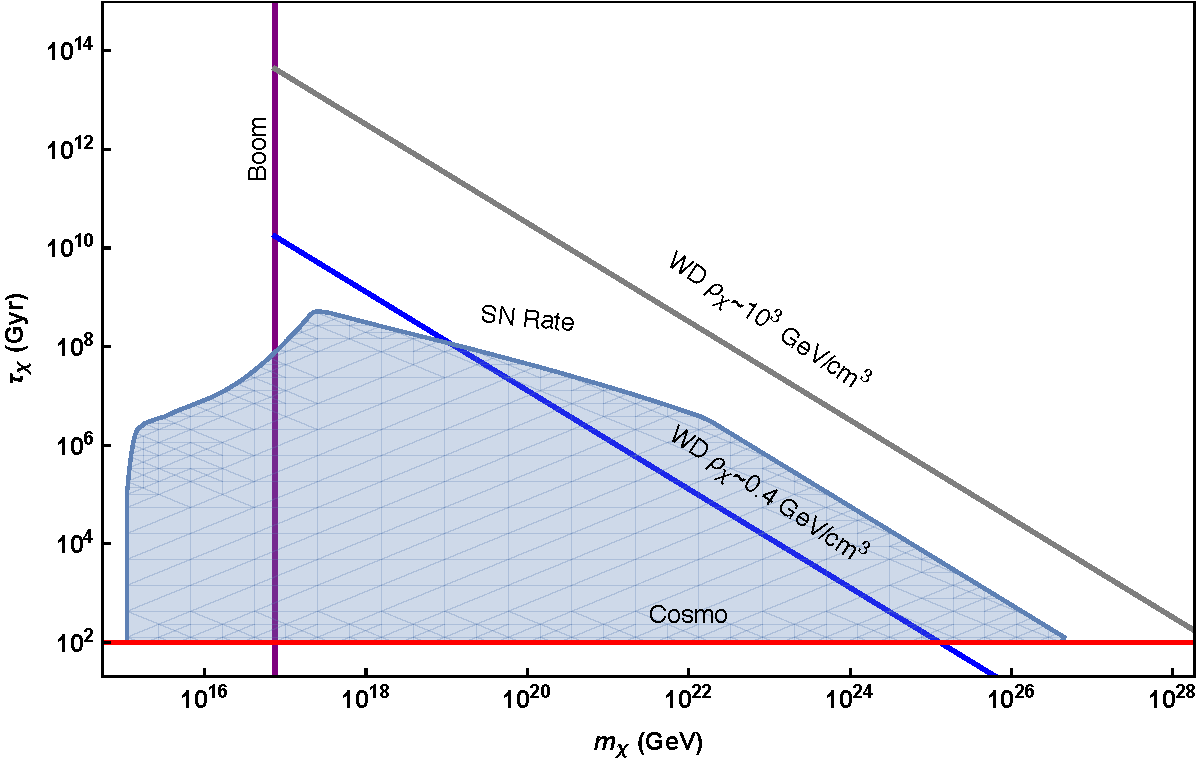
\includegraphics[scale=.45]{decayobservation.pdf}
\caption{Constraints on DM decay lifetime into photons with $\eta =1$. Bounds come from observations of a single WD (local and galactic center) and measured SN rate}
\label{fig:decayclasses}
\end{figure}
 
\subsection{Transit Constraints}
\label{sec:TransitConstraints}

The DM transit rate through a WD (including a gravitational Sommerfeld enhancement) is given by
\begin{align}
\Gamma_\text{transit} \sim \frac{\rho_{\text{DM}}}{m_\text{DM}} R_\text{WD}^2 \l\frac{v_\text{esc}}{v}\r^2 v.
\label{eq:TransitFluxCondition}
\end{align}
In order to constrain a DM model through its transit interaction with a WD, we require that it satisfy the explosive condition \eqref{eq:transitexplosion}. 
This is given in terms of an LET, which parameterizes the ability for DM to release sufficient energy to the star in the form of SM particles.
$(dE/dx)_\text{LET}$ for any realistic DM model would necessarily involve a sum over stellar targets along with species that could be produced, as well as an integral over the produced particle spectrum.
However, consider a simplified interaction in which $\sigma_{i,\epsilon}$ denotes the cross section for DM to scatter off a stellar constituent, producing $N_i$ SM particles of species $i$ and each with kinetic energy $\epsilon$.
If this were the only available channel for the DM to deposit energy, then its LET could be written as
\begin{align}
\label{eq:schematicLET}
  \left( \frac{d E}{d x} \right)_\text{LET} = n_\text{ion} \cdot N_i \sigma_{i,\epsilon} \epsilon,
\end{align}
where we now specify to the case of DM collisions with nuclear targets. 
With such a schematic for the DM-SM scattering interaction, the transit heating length for the process can be explicitly calculated using the results of Section~\ref{sec:SMHeating}.

In addition, we also make a sensible assumption that the LET $(dE/dx)_\text{LET}$ and DM stopping power $(dE/dx)_\text{SP}$ are equal for fixed number density - that is, the DM loses kinetic energy at the same rate as energy is deposited to the WD.
While such a statement is certainly not true for all DM models (such as the Q-ball, which liberates binding energy rather than transferring kinetic energy), it provides a useful benchmark to express constraints.
With this assumption, it is interesting to note that combining the transit explosion condition \eqref{eq:transitexplosion} with $\eqref{eq:schematicLET}$ yields a lower bound on DM mass such that the DM is able to both penetrate the crust \emph{and} trigger an explosion:
\begin{align}
\label{eq:transitmass}
m_{\text{DM}} >  T_f \lambda_T^2 \l \frac{n_{\text{crust}} R_{\text{crust}}}{v_{\text{esc}}^2} \r.
\end{align}
For typical WD parameters we find that the DM mass must be greater than $\sim 10^{27} ~\GeV$, taking the density of the WD crust $n_\text{crust}$ to be a nominal $\OO(10^{-2})$ fraction of the central density $n_\text{ion}$ \textcolor{blue}{cite}. 
In other words, if \eqref{eq:transitmass} were violated then the DM interaction is either not strong enough to ignite the WD or it is so strong that it does not penetrate the crust without losing appreciable kinetic energy.
However, it is important to note that this bound is only applicable when the energy input to the WD is chiefly coming from the DM kinetic energy, rather than binding energy or other sources.
With the above schematic for a DM transit, we constrain the parameter $\sigma_{i,\epsilon} \epsilon$ as a function of DM mass $m_\text{DM}$ - for simplicity, we take a single SM particle released per interaction $N_i = 1$. 
This is done in Figures \ref{fig:transitclasses}, \ref{fig:transitepsilon}, and \ref{fig:transitspecies} using the different classes of observation available and for representative choices of $\epsilon$ and SM species $i$ released.

\begin{figure}
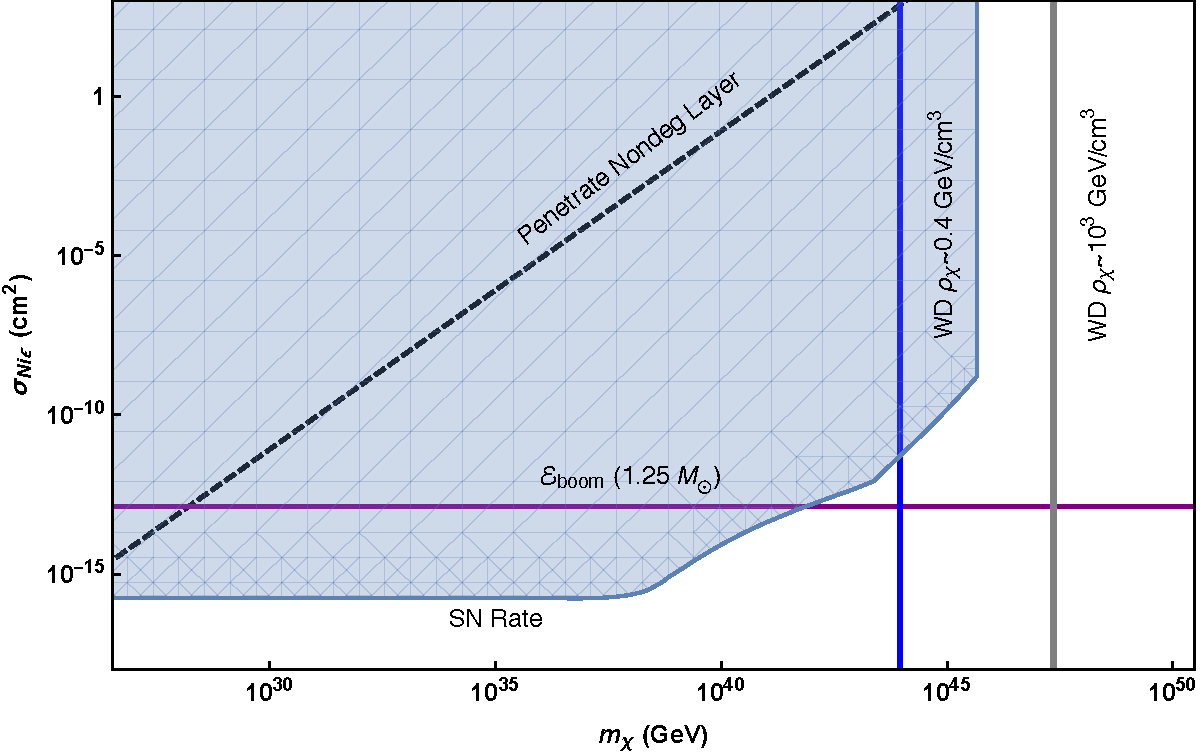
\includegraphics[scale=.45]{transitobservation.pdf}
\caption{Constraints on DM-nuclei scattering cross section to produce photons of energy $\epsilon = \text{TeV}$. Bounds come from observations of a single WD (local and galactic center) and measured SN rate}
\label{fig:transitclasses}
\end{figure}

\section{Q-balls}
\label{sec:QBalls}

Having derived generic constraints on models of ultra-heavy DM in Section~\ref{sec:Constraints}, we turn towards a more concrete example: Q-balls.
In various supersymmetric extensions of the SM, non-topological solitons called Q-balls can be produced in the early universe \cite{Coleman:1985ki, Kusenko:1997si}.
If these Q-balls were stable, they would comprise a component of the DM today.
For gauge-mediated models with flat scalar potentials, the Q-ball mass and radius are given by
\begin{equation}
\label{eq:Qballprop}
M_Q \sim m_S Q^{3/4}, ~~~ R_Q \sim m_S^{-1} Q^{1/4},
\end{equation}
where $m_S$ is related to the scale of supersymmetry breaking.
The condition $M_Q/Q < m_p$ ensures that the Q-ball is stable against decay to nucleons \cite{Dine:2003ax}.
When an (electrically neutral) baryonic Q-ball interacts with a nucleon, it absorbs its baryonic charge as a minimum-energy configuration and induces the dissociation of the nucleon into free quarks.
During this process, $\sim \text{GeV}$ of energy is released through the emission of 2 - 3 pions \cite{Dine:2003ax}.
We assume that for each Q-ball collision, there is equal probability to produce $\pi^0$ and $\pi^\pm$ under the constraint of charge conservation.
The cross section for this interaction is approximately geometric:
\begin{align}
\sigma_Q \sim \pi R_Q^2.
\end{align}
Note that a sufficiently massive Q-ball will become a black hole if the Q-ball radius is less than the Schwarzschild radius $R_Q \lesssim G M_Q$.
In the model described above, this translates into a condition $(M_\text{pl}/m_S)^4 \lesssim Q$.
For Q-ball masses of this order, gravitational interactions become relevant.

We now determine the explosiveness of a Q-ball transit.
In the notation of Section \ref{sec:Constraints}, this process is described by the parameter $(dE/dx)_\text{LET} \sim n_\text{ion} \cdot N_\pi \sigma_Q \epsilon$, where the nuclear interaction results in $N_\pi \sim 30$ pions released, each with kinetic energy $\epsilon \sim 500 ~\text{MeV}$.
Numerous experiments have studied interactions of pions in this energy range incident upon complex nuclei targets such as carbon.
It is found that there is roughly equal cross section of order $\OO (100 ~\text{mb})$ for a (neutral or charged) pion to either elastically scatter or become absorbed in a nonelastic scatter with no final state pion \cite{Pionnuclear}.
As seen in Section \ref{sec:SMHeating}, nonelastic collisions are most relevant for energy loss and will induce a hadronic shower.
The corresponding heating length of the Q-ball interaction is computed in a straightforward manner $L_0 \sim \text{few} \times 10^{-7} ~\text{cm}$ in WD density of $n_\text{ion} \sim 10^{32} ~\text{cm}^{-3}$.
If the Q-ball cross section is related to its mass and baryonic charge as in \eqref{eq:Qballprop}, we find that $Q \gtrsim 10^{38} \l\frac{m_S}{\text{TeV}}\r^4$ is capable of triggering runaway fusion in a heavy $\sim 1.25 ~M_{\odot}$ WD.
Note that for such large values of $Q$ there is negligible stopping power for the Q-ball to slow down in a WD, and as such condition \eqref{eq:CrustCondition} will be trivially satisfied.

Currently, the strongest constraints on Q-balls come from large detectors, i.e. Super-Kamiokande as well as air fluorescence detectors of cosmic rays
However, the constraints possible with the WD detector are in a fundamentally inaccessible region of parameter space for these terrestrial-based experiments due to the extremely low flux, and thus our new constraints are wholly complementary.
The strongest proposed limits due to the existence of a heavy WD in the galactic center are plotted in Figure~\ref{fig:Qballconstraint}. As a comparison, the combined limits from Super-K and the OA,TA cosmic ray detectors are shown in red. 
\begin{figure}
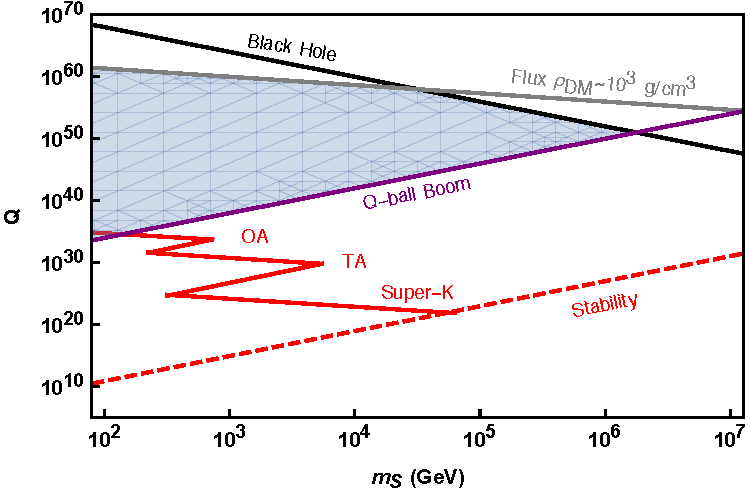
\includegraphics[scale=.55]{Qballconstraint.pdf}
\caption{Constraints on baryonic Q-balls from transits of a $\sim 1.25 ~M_{\odot}$ WD in the galactic center. Also shown are the limits from Super-K and the OA, TA cosmic ray detectors, and the lower bound on $Q$ for which the Q-ball is stable against decay to nucleons.}
\label{fig:Qballconstraint}
\end{figure}

\section{Discussion}
\label{sec:Discussion}

\begin{appendices}

\section{Particle Interactions in a White Dwarf}
\label{sec:appendix}
Here we provide a detailed analysis of the possible electromagnetic and strong interactions in a WD.
This is primarily aimed towards calculating the stopping of high-energy electrons, photons, and light hadrons (protons, neutrons, pions) within the stellar medium, the results of which are summarized in Figures \ref{fig:SPelectron}, \ref{fig:SPphoton}, \ref{fig:SPnuc}, and \ref{fig:SPpion}.
The interior of a WD is a complex environment (unless otherwise noted, we will assume a carbon-oxygen WD).
Famously, the star is supported against collapse by electron degeneracy pressure with a characteristic Fermi energy
\begin{equation}
E_F \sim (3 \pi^2 n_e)^{1/3} \sim 0.1 - 1 ~\text{MeV}
\end{equation}
where $n_e$ is the number density of electrons.
The nuclei are at an ambient temperature $T \sim \text{keV}$ and form a strongly-coupled plasma with lattice energy
\begin{equation}
\label{eq:lattice}
\omega \sim \frac{Z^2 \alpha}{n_\text{ion}^{-1/3}} \sim 10^{-2} - 10^{-1} ~\text{MeV}
\end{equation}
where $n_\text{ion}$ is the number density of nuclei \cite{Teukolsky}. 
\begin{figure}
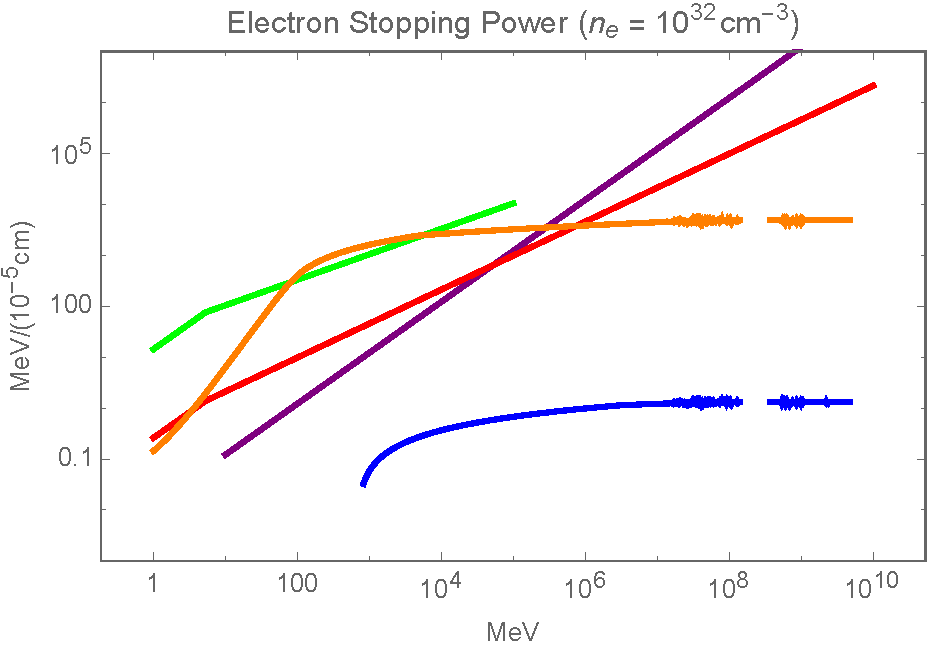
\includegraphics[scale=.45]{SPelectron.pdf}
\caption{Electron energy loss in a WD density $n_e = 10^{32} ~\text{cm}^{-3}$ For $n_e \gtrsim 10^{32} ~\text{cm}^{-3}$, bremsstrahlung and pair production contributions should be ignored}
\label{fig:SPelectron}
\end{figure}
\begin{figure}
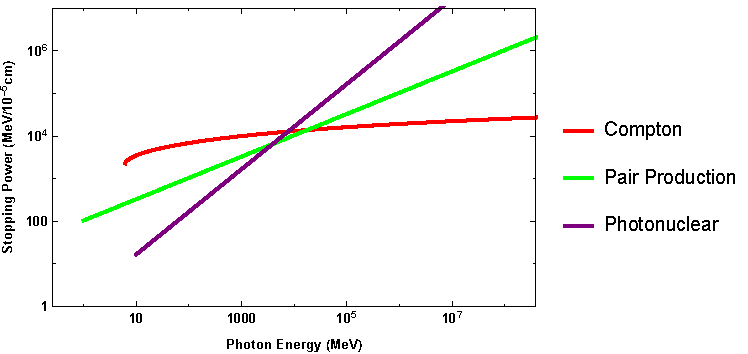
\includegraphics[scale=.45]{SPphoton.pdf}
\caption{Photon energy loss in a WD density $n_e = 10^{32} ~\text{cm}^{-3}$ For $n_e \gtrsim 10^{32} ~\text{cm}^{-3}$, bremsstrahlung and pair production contributions should be ignored}
\label{fig:SPphoton}
\end{figure}
\begin{figure}
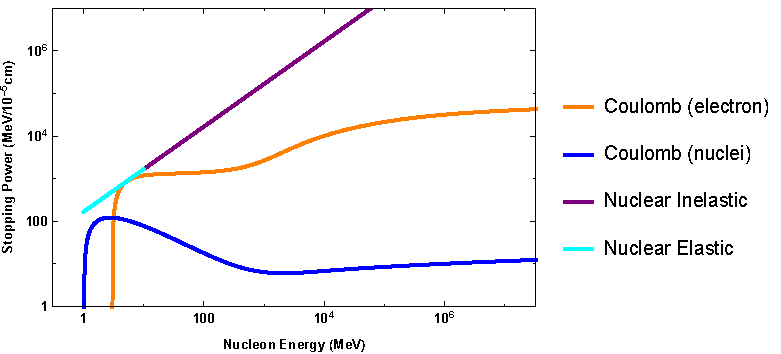
\includegraphics[scale=.45]{SPnucleon.pdf}
\caption{Nucleon energy loss in a WD with density $n_e = 10^{33} ~\text{cm}^{-3}$. The Coulomb stopping powers apply only to protons.}
\label{fig:SPnuc}
\end{figure}
\begin{figure}
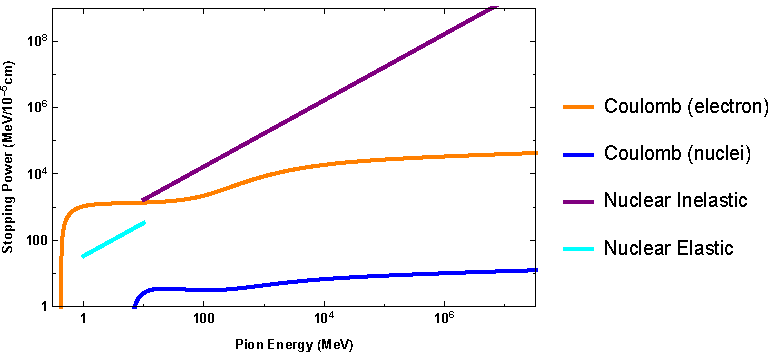
\includegraphics[scale=.45]{SPpion.pdf}
\caption{Pion energy loss in a WD with density $n_e = 10^{33} ~\text{cm}^{-3}$. The Coulomb stopping powers apply only to charged pion.}
\label{fig:SPpion}
\end{figure}

\subsection*{Coulomb Collisions}

An incident particle of mass $m$, charge $e$, and velocity $\beta$ scattering off a stationary target of mass $M$, charge $Ze$ at impact parameter $b$ will transfer energy
\begin{equation}
\label{eq:impact}
E' \sim \frac{Z^2 \alpha^2}{b^2 \beta ^2 M},
\end{equation}
valid for small energy transfers less than the mass of the target. 
The differential cross section for the interaction is given by the Rutherford cross section
\begin{equation}
\label{eq:rutherford}
\frac{d \sigma}{dE'} = \frac{2 \pi  \alpha^2 Z^2}{M \beta^2} \frac{1}{E'^2},
\end{equation}
where we have assumed a sufficiently fast incident particle so that interactions are governed by single collisions with energy transfer $E'$ \cite{Agashe:2014kda}.
In the case of a target electron, the full QED calculation yields a cross section of similar form
\begin{equation}
\frac{d \sigma}{dE'} = \frac{2 \pi  \alpha^2 Z^2}{m_e \beta^2} \frac{1}{E'^2} \l1-\beta^2 \frac{E^\prime}{E_\text{kin}} \r,
\end{equation}
where $E_\text{kin}$ is the maximum possible energy transfer satisfying kinematic constraints in a backward scatter. For a target electron, this is simply:
\begin{equation}
\label{eq:Ekin}
E_{\text{kin}} = \frac{2 m_e \beta^2 \gamma^2}{1+ 2\gamma m_e/m +(m_e/m)^2}.
\end{equation}
It is straightforward to understand the parametric dependences of \eqref{eq:rutherford}: there is increased likelihood to scatter for slowly moving incident particles undergoing soft-scatters against lighter targets.
Therefore, one would expect that soft-scattering dominates the energy loss, and that collisions with nuclei of mass $M$ are suppressed $\OO\l\frac{Z m_e}{M}\r$ as compared to collisions with electrons.
While this is certainly true for incident charged particles in non-degenerate matter, these expectations turn out to be false when considering scattering off a degenerate species.

We first compute the energy loss of high-energy charged particles via Coulomb scattering off nuclear targets. 
In this case, the stopping power is given by:
\begin{align}
\label{eq:SP}
-  \l \frac{dE}{dx}\r \sim \frac{n_\text{ion} Z^2 \alpha^2}{M \beta^2} \log {\l\frac{E_{\text{max}}}{E_{\text{min}}}\r}.
\end{align}
We take the upper limit $E_\text{max}$ to be the maximum energy transfer allowed kinematically. 
The minimum energy transfer $E_\text{min}$ is set by the impact parameter at which charge screening becomes relevant. 
In a WD, the degenerate electron gas exponentially screens Coulomb interactions at distances larger than the Thomas-Fermi length:
\begin{equation}
\label{eq:TF}
\lambda_{\text{TF}} = \l \frac{6 \pi Z \alpha n_e}{E_F}\r^{-1/2}.
\end{equation}
In addition, for energy transfers greater than $\omega$, the lattice structure of ions in the WD introduces further complications.
In particular, momentum transfers from collisions below this threshold will lead to suppressed energy loss due to collective effects.
We set the lower bound on Coulomb scattering off nuclear targets (not applicable for electron targets) to be $\sim \omega$ so that we only account for energy transfers greater than the ion lattice binding energy.
At lower energies, we estimate the stopping power into phonon excitations as follows: \textcolor{blue}{paragraph on phonons}

Now consider Coulomb collisions with degenerate electrons.
While a proper treatment of this interaction would also take into account the relativistic motion of the degenerate electron gas, this will introduce a minor correction for highly relativistic incident particles. 
An incident particle transferring energy $E'$ can only scatter those electrons within $E'$ of the Fermi surface.
We define a modified density of electrons $n_e(E')$ as:
\begin{equation}
\label{eq:pauliblocking}
n_e(E') = \left\{
        \begin{array}{ll}
            \displaystyle \int \limits_{E_F -E'}^{E_F}dE ~g(E) & \quad E_F > E' \\
            n_e & \quad E_F < E'
        \end{array}
    \right.,
\end{equation}
where $g(E)$ is the density of states per unit volume for a three-dimensional free electron gas.
The effect of degeneracy can also be cast as a suppression of the differential cross section of order $\mathcal{O}(E'/E_F)$ whenever energy less than the Fermi energy is transferred.
Therefore, unlike in the non-degenerate case, the Pauli-suppressed energy loss due to soft-scatters are in fact subdominant to the contributions from rare hard-scatters.
This stopping power is also sensitive to the integration bounds $E_{\text{max}}$ and $E_{\text{min}}$ as a power-law dependence unlike the logarithmic sensitivity \eqref{eq:SP} in the case of a non-degenerate target.

\subsection*{Compton and Inverse Compton Scattering}
Photons and charged particles can elastically exchange energy through Compton scattering.
We focus first on an incident photon losing energy to the WD medium.
Since the cross section for this process scales inversely with the target mass, the stopping due to photon-ion collisions will be subdominant to photon-electron collisions and we ignore the former. 
Consider an incident photon of energy $k$ scattering off an electron of energy $E \sim E_F$.
In the rest frame of the electron, this cross section is given by the Klein-Nishina formula
\begin{equation}
\label{KN}
  \frac{d\sigma_\text{KN}}{d (\cos \theta)} = \frac{\pi \alpha^2}{m_e^2} 
  \l \frac{k^\prime}{k} \r^2 
  \l \frac{k^\prime}{k} + \frac{k}{k^\prime} -\sin^2 \theta \r
\end{equation}
where $k^\prime$ is the outgoing photon energy, related to the scattering angle $\theta$ by Compton's formula
\begin{equation}
{k^{\prime }={\frac {k}{1+{\frac {k}{m_e}}(1-\cos \theta )}}}.
\end{equation}
In the limit $k > m_e$, the cross section is suppressed by the incoming energy $\sigma \sim \frac{\alpha^2}{m_e k}$. 
The outgoing photons will scatter predominately in a near-forward direction, $\cos \theta \approx m_e/k$, with an energy loss $k^\prime \sim m_e$.
Thus the typical photon energy loss is large, $\Delta k \sim m_e - k$, and cooling proceeds via a small number of hard scatters.
The stopping power is roughly:
\begin{equation}
\label{eq:approx-comptonSP}
  - \l\frac{dk}{dx}\r \sim n_e \sigma \Delta{k} 
  \sim n_e \frac{\alpha^2}{m_e} \l 1 - \frac{m_e}{k} \r.
\end{equation}
A more careful analysis computes the stopping power as 
\begin{equation}
\label{eq:comptonSP}
  -\l\frac{dk}{dx}\r =  \int d (\cos \theta) n_e \frac{d\sigma_\text{KN}}{d (\cos \theta)} \l k - k^\prime \r, 
\end{equation}
taking into account the Lorentz boost to the electron's rest frame.
This does not alter the result beyond $\OO(1)$ factors, since the target electrons are only slightly relativistic.
Further, Pauli-blocking of the target electrons should be taken into account via \eqref{eq:pauliblocking}, although we find that degeneracy only introduces a significant suppression when $k \lesssim 10 ~\text{MeV}$.
This is also expected, as the interaction is dominated by hard, near-forward scatters.

We now briefly consider incident electrons which may cool by (inverse) Compton scatters with the thermal bath of photons in the WD.  
The number density of these photons is set by the temperature of the star $n_\gamma \sim T^3 \sim 10^{23} ~\cm^{-3}$, where we have taken $T \sim \text{keV}$. 
Since this is roughly ten orders of magnitude less than the the ions and electron densities in the WD, it is reasonable to suspect that the energy loss due to inverse Compton scattering is far subdominant to electron-electron or even electron-ion collisions. 
An estimate in the manner of the above calculation (including the now-significant boost factors) gives the inverse Compton stopping power in terms of the photon temperature $T$ and incident electron energy $E$:  
\begin{equation}
\label{eq:invcomptonSP}
  -\l \frac{dE}{dx}\r \sim 
  \begin{cases}
    \alpha^2 \frac{T^4}{m_e^4} E^2 & E \lesssim \frac{m_e^2}{T} \\
    \alpha^2 T^2 & E \gtrsim \frac{m_e^2}{T} \\
  \end{cases},
\end{equation}
where the change in scaling with $E$ marks a transition from Thompson-like scattering in the electron rest frame to suppressed high-energy scattering.
As expected, we find that the inverse Compton stopping power is negligible as compared to other forms of energy loss such as Coulomb scattering. 

\subsection*{Bremsstrahlung and Pair Production with LPM Suppression}
Bremsstrahlung and pair production can be significant sources of energy loss for high-energy electrons and photons. We restrict our attention to radiative processes off target nuclei rather than target electrons as the latter are additionally suppressed by degeneracy, kinematic recoil, and charge factors. 
The cross section for an electron of energy $E$ to radiate a photon of energy $k$ is given by the Bethe-Heitler formula
\begin{equation}
\label{eq:BH}
\frac{d \sigma_\text{BH}}{dk} = \frac{1}{3 k n_\text{ion} X_0} (y^2+2 [1+ (1-y)^2]), ~~~ y = k/E.
\end{equation}
$X_0$ is the radiation length, and is generally of the form
\begin{equation}
\label{eq:radiationlength}
X_0^{-1} = 4 n_\text{ion} Z^2 \frac{\alpha^3}{m_e^2} \log{\Lambda}, ~~~ \log{\Lambda} \sim \int \limits_{b_\text{min}}^{b_\text{max}} \frac{1}{b}.
\end{equation}
where $\log{\Lambda}$ is a logarithmic form factor containing the maximum and minimum effective impact parameters allowed in the scatter.
Integrating \eqref{eq:BH}, we find the energy loss due to bremsstrahlung is simply 
\begin{equation}
-\l\frac{dE}{dx}\r \sim \frac{E}{X_0}.
\end{equation}

$b_\text{min}$ in \eqref{eq:radiationlength} is set by a quantum-mechanical bound such that the radiated photon frequency is not larger than the initial electron energy. 
For a bare nucleus, this distance is the electron Compton wavelength $b_\text{min} = \lambda_e = \frac{1}{m_e}$. \textcolor{red}{another sentence to clarify}
It is important to note that collisions at impact parameters \emph{less} than $b_\text{min}$ will still radiate, but with exponentially suppressed intensity.
Classically, this is manifested by the decoherence of radiation at large scattering angles.
$b_\text{max}$ is set by the distance at which the nuclear target is screened.
For an atomic target this is of order the Bohr radius, and in the WD this is the Thomas-Fermi length \eqref{eq:TF}.
Evidently, there exists a critical electron number density $n_e \sim 10^{32} ~\text{cm}^{-3}$ at which the logarithmic form factor vanishes.
For our purposes, we simply take $\log{\Lambda} \sim \OO(1)$ whenever $b_\text{min} \lesssim b_\text{max}$ while effectively ignoring the energy loss due to bremsstrahlung in a sufficiently dense WD.

However, bremsstrahlung will be suppressed by the ``Landau-Pomeranchuk-Migdal" (LPM) effect - see \cite{Klein:1998du} for an extensive review.
High-energy radiative processes involve very small longitudinal momentum transfers to nuclear targets ($\propto k/E^2$ in the case of bremsstrahlung).
Quantum mechanically, this interaction is delocalized across a formation length over which amplitudes from different scattering centers will interfere.
This interference turns out to be destructive and must be taken into account in the case of high energies or high-density mediums.
Calculations of the LPM effect can be done semi-classically based on average multiple scattering.
It is found that bremsstrahlung is suppressed for $k < E(E-k)/E_\text{LPM}$, where
\begin{equation}
\label{eq:LPM}
E_\text{LPM} = \frac{m_e^2 X_0 \alpha}{4 \pi}.
\end{equation}
For the WD densities in which radiative energy loss is considered, $E_\text{LPM} \sim 10-10^{3} ~\text{MeV}$.
The degree of suppression is found to be
\begin{equation}
\frac{d\sigma_\text{LPM}/dk}{d\sigma_\text{BH}/dk} = \sqrt{\frac{k E_\text{LPM}}{E (E-k)}},
\end{equation}
so that the bremsstrahlung stopping power in the regime of high-suppression is modified
\begin{equation}
\label{eq:bremloss}
-\l\frac{dE}{dx}\r_\text{LPM} \sim \l\frac{E_\text{LPM}}{E} \r^{1/2} \frac{E}{X_0}, ~~~ E>E_\text{LPM}.
\end{equation}
We find that the LPM effect diminishes energy loss due to soft radiation so that the radiative stopping power is dominated by single, hard bremsstrahlung.

In addition to the LPM effect, other forms of interaction within a formation length will suppress bremsstrahlung when $k \ll E$.
The emitted photon can coherently scatter off electrons and ions in the media, acquiring an effective mass of order the plasma frequency $\omega_p$.
Semi-classically, this results in a suppression of order $(k/\gamma \omega_p)^2$ when the radiated photon energy $k < \gamma \omega_p$.
This is known as the ``dielectric effect".
For high-energy electrons, this dielectric suppression only introduces a minor correction to \eqref{eq:bremloss}, in which soft radiation is already suppressed by the LPM effect \cite{Klein:1998du}.

We now briefly summarize the stopping of photons via pair production. Similar to \eqref{eq:BH}, the cross section for a photon of energy $k$ to produce an electron-positron pair with energies $E$ and $k-E$ is
\begin{equation}
\label{eq:PP}
\frac{d \sigma_\text{BH}}{dE} = \frac{1}{3 k n_\text{ion} X_0} (1+ 2[x^2+ (1-x)^2]) ~~~ x = E/k,
\end{equation}
valid beyond the threshold energy $k \gtrsim m_e$. 
As a result, the pair production cross section $\sim 1/(n_\text{ion} X_0)$.
However, the LPM effect suppresses pair production at energies $E(k-E) > k E_\text{LPM}$ so that the cross section reduces to
\begin{equation}
\sigma_{pp} \sim \l\frac{E_\text{LPM}}{k} \r^{1/2} \frac{1}{n_\text{ion} X_0}, ~~~ E>E_\text{LPM}.
\end{equation}

Note that the LPM effect is less significant for higher-order electromagnetic processes since these generally involve larger momentum transfers for the same final-state kinematics.
Thus, when the suppression factor exceeds $\OO(\alpha)$, these interactions should also be considered.
For instance, the energy loss due to electron direct pair production $e^-N \to e^+ e^- e^- N$ has been calculated in \cite{Gerhardt:2010bj} and is found to exceed that of bremsstrahlung at an energy $\sim 10^{8} ~\GeV$. 
A similar crossover is to be expected for other higher-order diagrams as well, although such a calculation is beyond the scope of this work. 
Rather, it is expected that at such high energies the stopping power is dominated by photonuclear and electronuclear interactions anyway, and we may simply ignore the contributions from other radiative processes \textcolor{blue}{convo with Klein}. 

\subsection*{Nuclear Interactions}
Nuclear interactions can be either elastic or nonelastic - the nature of the interaction is largely determined by the incident particle energy.
Elastic collisions are most relevant at scales less than the nuclear binding energy, $E_\text{nuc} \sim 10 ~\text{MeV}$.
A single, backward elastic scatter could result in an incident particle losing virtually all of its energy if the incident and target masses are the same.
However, we will be primarily concerned with light hadrons incident on relatively heavy nuclei, i.e.
ping-pong balls bouncing around a sea of bowling balls.

An elastic collision between an incident (non-relativistic) mass $m$ with kinetic energy $\epsilon$ and a heavy, stationary target mass $M$ results in an energy transfer
\begin{equation}
\label{eq:elasticratio}
E' \approx \l \frac{2 m}{M}\r \epsilon, ~~~~ m < M,
\end{equation}
where it is assumed there is an isotropic distribution in the center-of-mass scattering angle.
Thus, a nucleon interacting with carbon nuclei transfers roughly 15\% of its incident energy after each elastic collision.
However, since the ions in a WD form a Coulomb lattice, elastic collisions cannot transfer energy less than \eqref{eq:lattice} without exciting phonon modes.
In the case of an incident nucleon, this limits the applicability of \eqref{eq:elasticratio} to energies $\epsilon \gtrsim \text{MeV}$.
The cross section for elastic scatters $\sigma_\text{el}$ has considerable dependence on the incident particle species and energy.
At energies below $\sim \text{MeV}$, $\sigma_\text{el}$ effectively vanishes for protons.
In the case of neutrons, $\sigma_\text{el}$ is roughly constant below $\sim \text{MeV}$ but is of a complicated form in the intermediate regime $1 - 10 ~\text{MeV}$ due to various nuclear resonances \textcolor{blue}{cite}.
For our purposes, we assume the elastic cross section for any hadron to be constant $\sigma_\text{el} \sim 1 ~\text{b}$ when $\epsilon \gtrsim \text{MeV}$.

Next we consider nonelastic collisions at incident energies $\epsilon \gtrsim E_\text{nuc}$.
In this regime, a nuclear collision generally results in an $\OO(1)$ number of energetic secondary hadrons (i.e.
protons, neutrons, pions, etc.) emitted roughly in the direction of the primary particle.
These secondary particles approximately split the initial total energy of the absorbed primary particle and can collide with other nuclei in the WD.
The remnant nucleus will generally be left in an excited state and relax through the emission of $\OO(10 ~\text{MeV})$ hadrons (``nuclear evaporation") and photons \cite{Rossi}.
A hadronic shower is the result of all such reactions caused by primary and secondary particles.
For simplicity, we take the nuclear mean free path for a light hadron (proton, neutron, pion) to be constant in energy with characteristic cross section
\begin{equation}
l_\text{h,non} \sim  \frac{1}{n_\text{ion} \sigma_\text{non}}, ~~~~ \sigma_\text{non} \sim 100 ~\text{mb}.
\end{equation}
Note that the shower length is only logarithmically sensitive to the initial energy or number of secondaries, and is thus primarily set by the nuclear mean free path.
In this case, the cascade induced by a high-energy initial hadron is adequately described by a stopping power
\begin{equation}
\label{eq:nucshower}
-\l \frac{dE}{dx}\r \sim \frac{E}{l_\text{h,inel}},
\end{equation}
neglecting logarithmic factors of $\OO(1)$.
The shower will end once final-state hadrons reach a critical energy $E_c$ - this is either the scale at which an additional mechanism dominates the stopping power or the minimum energy required to induce further showers $E_\text{nuc}$.
Note that while neutrons and $\pi^\pm$ have characteristically long lifetimes, the mean distance traversed by a neutral pion before decaying to photons $\sim 10^{-7} - 10^{-6} ~\text{cm}$ for $\epsilon \sim 1 - 10 ~\text{MeV}$.
Hence, there are minimal electromagnetic contributions from $\pi^0$ decays during the progression of a hadronic cascade.

Energetic $k \gtrsim 10 ~\text{MeV}$ photons can also interact with nuclei and induce a hadronic shower.
There is considerable uncertainty in the evaluation of high-energy photonuclear cross sections, and a detailed model is beyond the scope of this work.
In fact at sufficiently high energies, photonuclear interactions can become coherent with the photon interaction spread over multiple nuclei \cite{Gerhardt:2010bj}.
This coherence will further reduce the photonuclear mean free path.
As a conservative estimate, we assume a constant photonuclear cross section in the relevant energy regime
\begin{align}
l_{\gamma, \text{non}} \sim \frac{1}{n_\text{ion} \sigma_{\gamma A}}, ~~~~ \sigma_{\gamma A} \sim 1 ~\text{mb}.
\end{align}
Similarly, charged leptons will lose energy via electronuclear interactions in which the incident particle radiates a virtual photon that then interacts hadronically with a nearby nucleus.
Note that a hadronic shower induced by electronuclear interactions are not affected by the LPM suppression \eqref{eq:LPM}.
Naively we expect the stopping power to be of order $\sim E \alpha/l_{\gamma, \text{non}}$.
A more detailed calculation \cite{Gerhardt:2010bj} differs from our naive estimate an $\OO(10)$ factor.
The largest uncertainty in calculating electronuclear stopping power at high energies is in evaluating hadronic cross sections, which require significant extrapolation from existing data and for which different models yield different results.





\end{appendices}

\section*{Acknowledgements}
We would like to thank D.Grabowska, K.Harigaya, S.R.Klein, R.McGehee, and J.Wurtele for stimulating discussions.
\textcolor{blue}{Grant acknowledgements}

\bibliography{Qballs}

\end{document}